\documentclass[a4paper, 10pt]{article}

\usepackage{fontspec}
\usepackage[hidelinks]{hyperref}
\usepackage[catalan]{babel}

\renewcommand*\contentsname{Índex}

\begin{document}
\title{Informe mecànic Projecte I}
\author{Marc Asenjo i Ponce de León \and
		Joan Marcè i Igual \and
		Iñigo Moreno i Caireta}
\date{\today}
\maketitle
\begin{center}
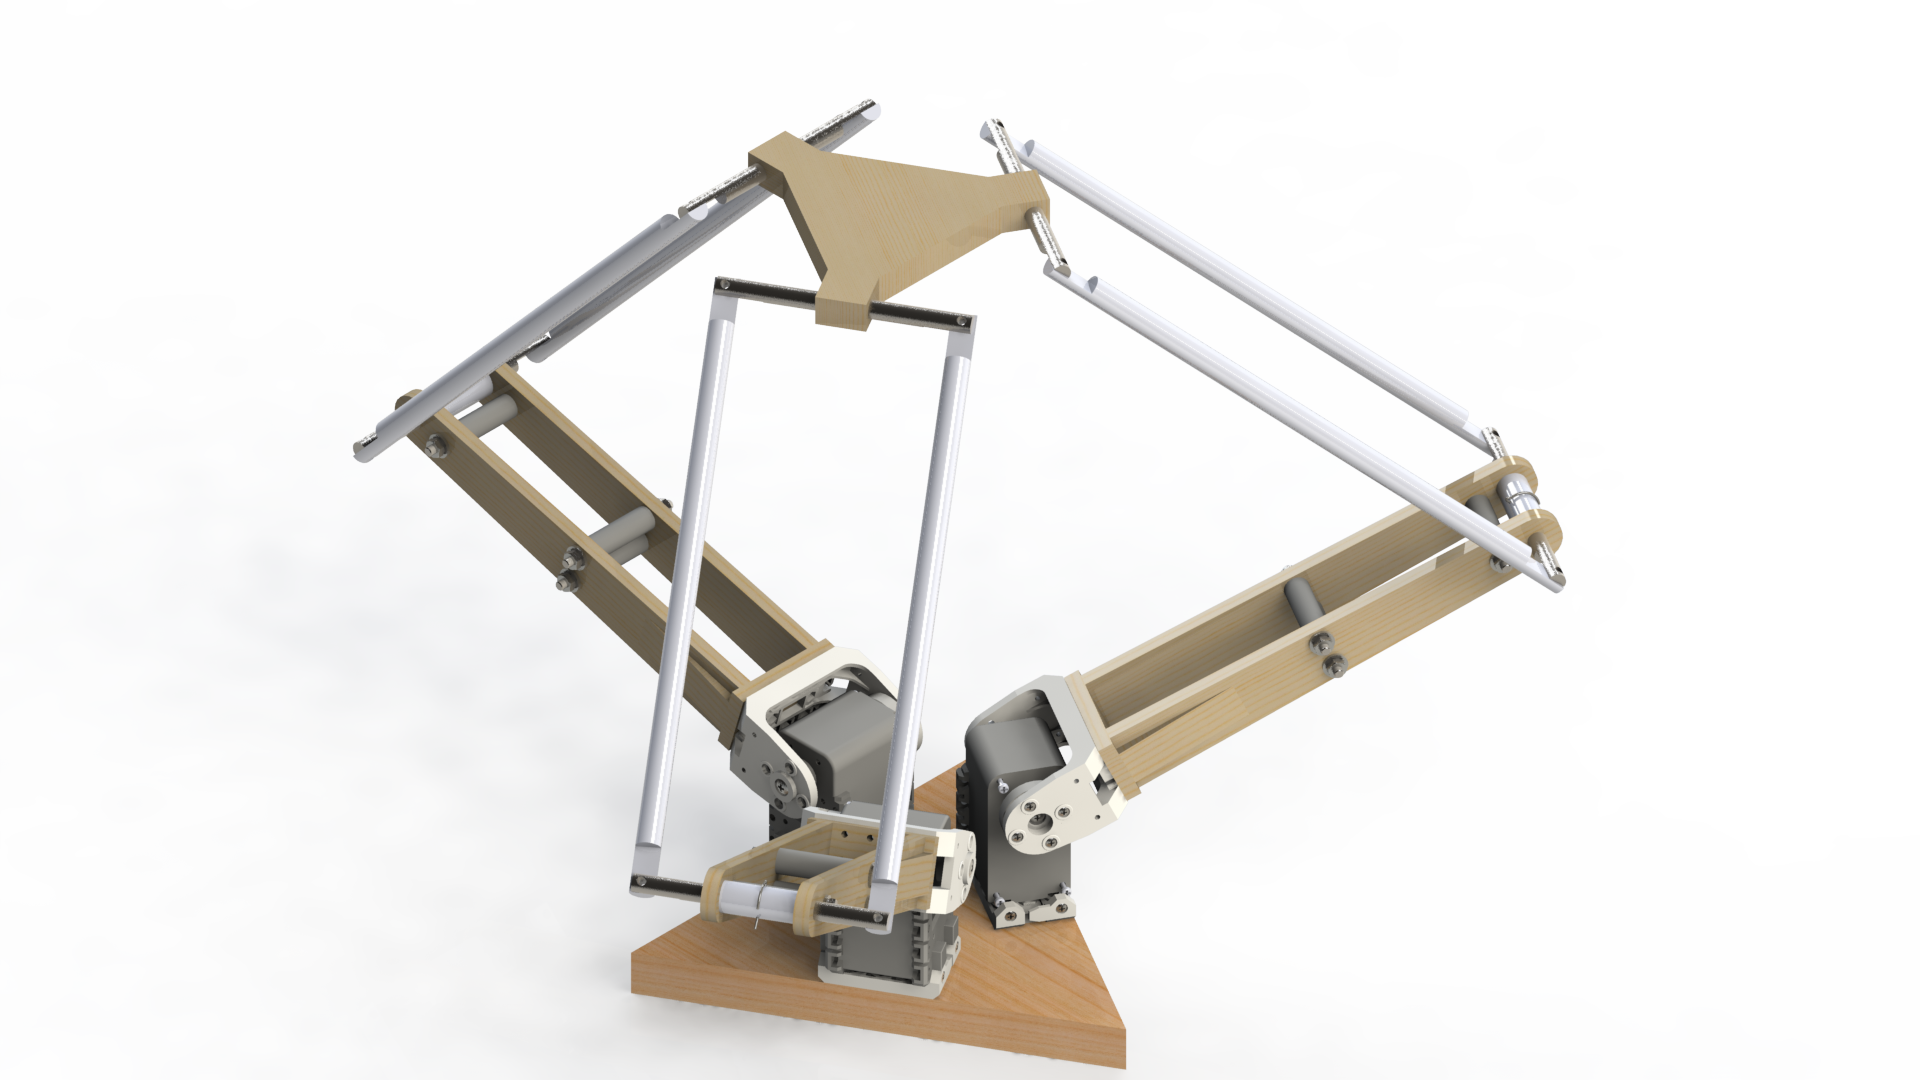
\includegraphics[width=0.5\textwidth]{./images/logo}
\end{center}

\newpage
\tableofcontents{}

\newpage
\section{Ensamblatge general}


\begin{figure}[h!]
\centering
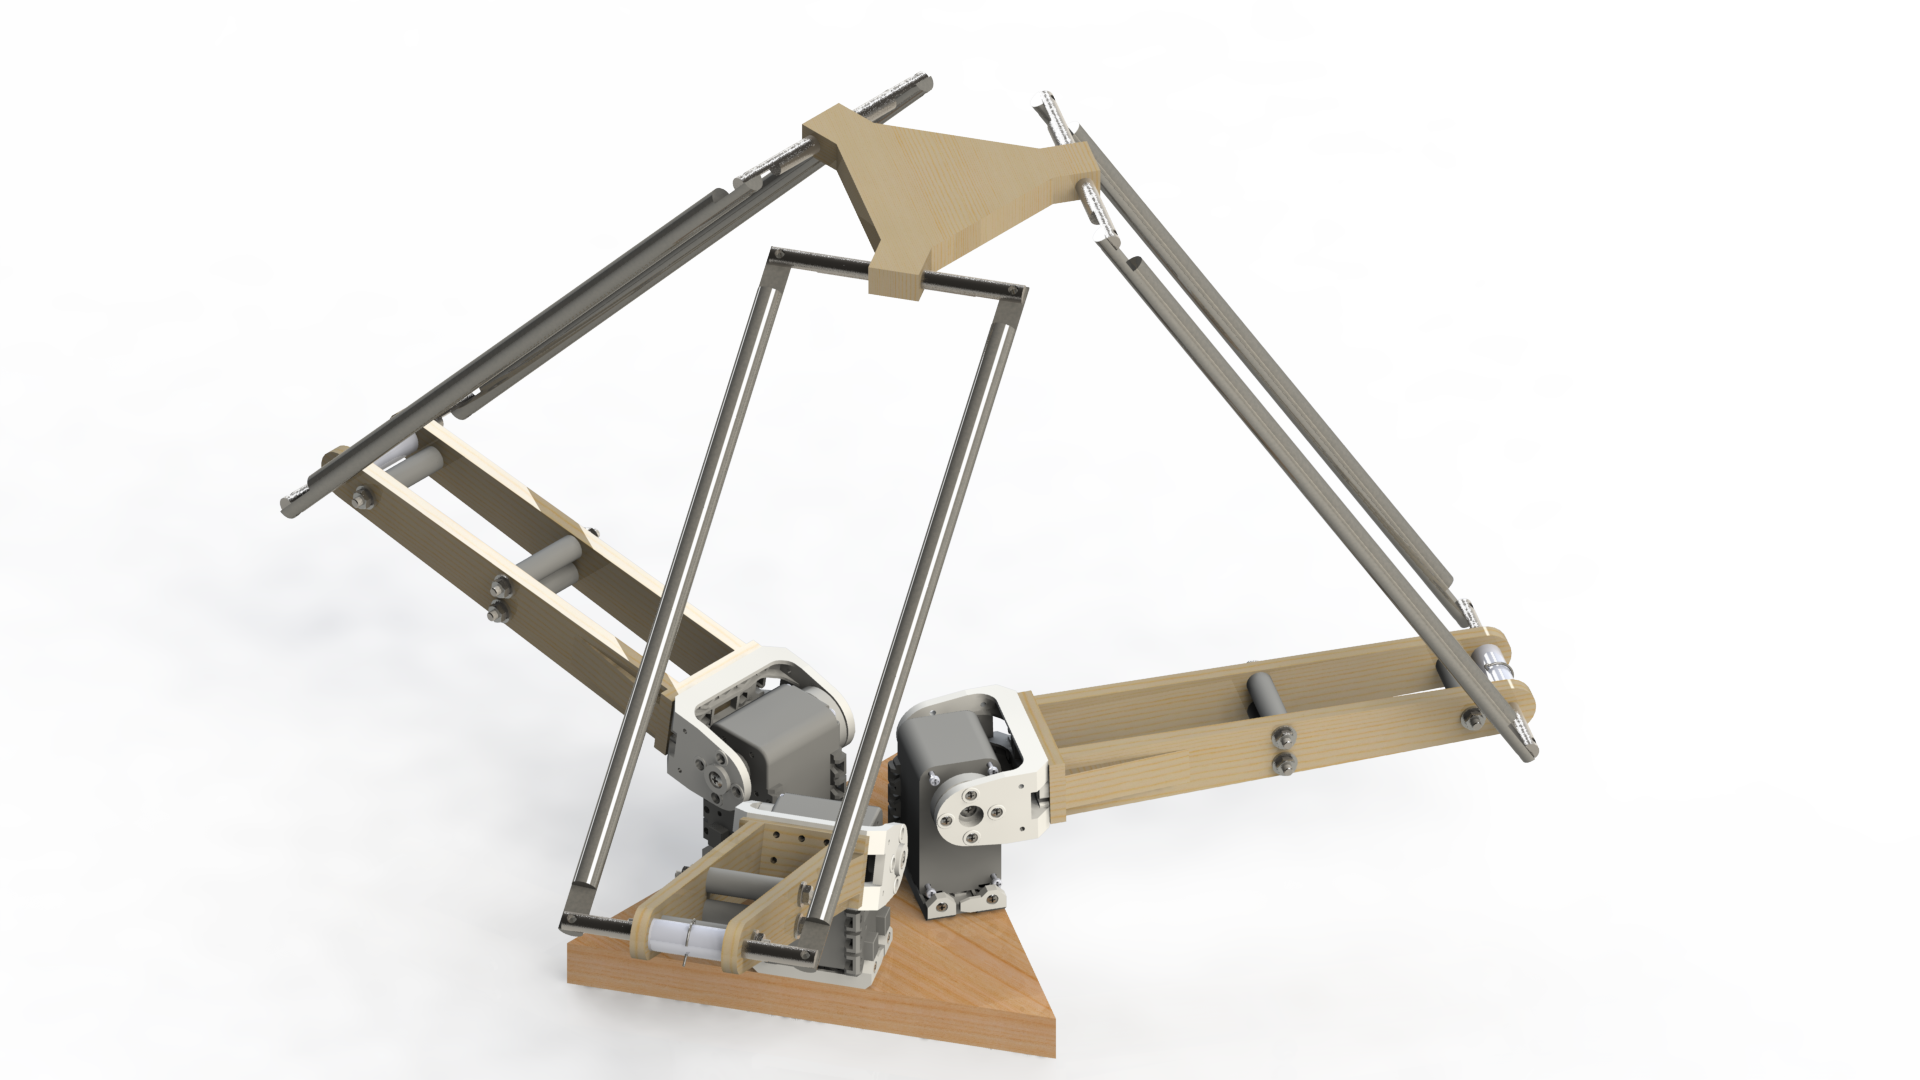
\includegraphics[width=10cm]{./images/general}
\end{figure}

Aquest robot delta està format per quatre parts generals; els servos, els braços, els avantbraços i la pinça final. 

El robot consta de tres servos que permetran el posicionament de la pinça; cada servomotor té acoblat un braç que es mou junt amb l'eix d'aquest. A més a més, els
braços estan units mitjançant un eix amb un avantbraç. Tots els avantbraços arriben a unir-se a la peça final que és la pinça permeten així que el moviment dels tres servos determini un punt a l'espai en el qual posicionar la pinça.


\newpage
\section{Servos}


\newpage
\section{Braç}

\subsection{Estructura}

\subsection{Estabilitzador}

\newpage
\section{Avantbraç}

\subsection{Vara}

\subsection{Alineador}

\subsection{Eix}

\subsection{Eix Pinça}

\subsection{Unió}

\newpage
\section{Pinça}

\end{document}